\begin{figure}[ht!]
	\begin{subfigure}{\linewidth}
		\caption{}
		\centering
		% include second image
		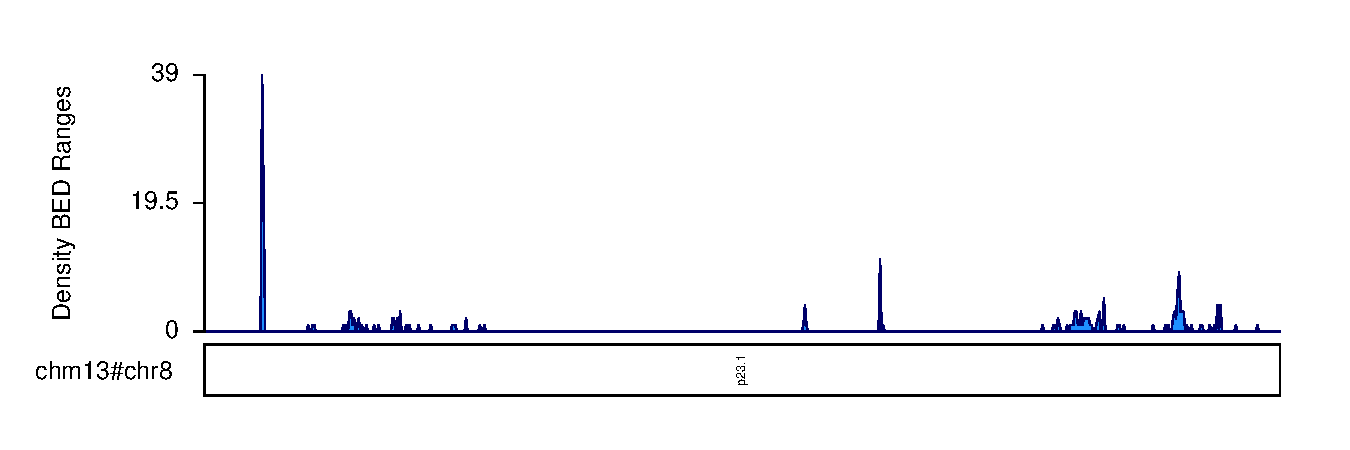
\includegraphics[width=1.0\linewidth, trim=0cm 2cm 0cm 2cm]{fig/tips/chr8_chm13_beta_defensin_locus_odgi_tips_w50000_karyoploteR}
		\label{fig:tips-karyo}
	\end{subfigure}
	\begin{subfigure}{\linewidth}
	\caption{}
	\centering
	% include second image
	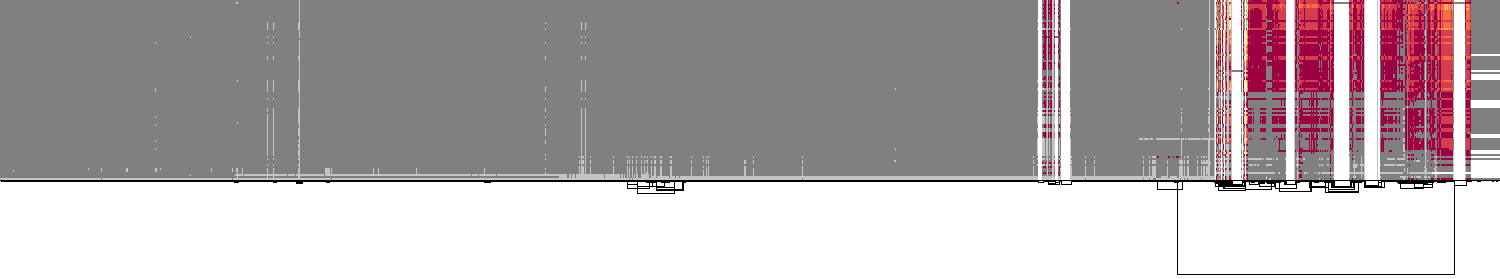
\includegraphics[width=1.0\linewidth, trim=-10cm 6cm -3.4cm 3cm]{fig/tips/chr8_pan_fa_c3d3224_7748b33.395c7f4_smooth_og_Y_og_p23_1_og_90paths_m}
	\label{fig:tips-viz}
\end{subfigure}
	%	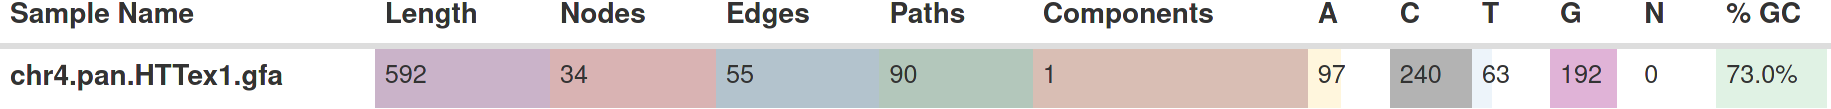
\includegraphics[width=\linewidth]{fig/metrics/chr4.pan.HTTex1.gfa.multiqc_odgi_stats.png}
	\caption{Visualizing the contigs of a beta-defensin locus pangenome graph. (\textbf{a}) Breakpoint ranges of the contigs in the beta-defensin locus pangenome graph of 90 haplotypes relative to CHM13. The \textit{odgi tips} results are visualized as the density of BED ranges across the whole \textit{p23.1} cytoband. The high peak at the beginning of \textit{p23.1} indicates that 39 contigs of the graph broke at this specific position relative to CHM13. (\textbf{b}) \textit{odgi viz} color by path depth visualization of the 90 longest paths in the beta-defensin locus pangenome graph including CHM13 and GRCh38 on the top: using the Spectra color palette with 4 levels of path depths. White, grey, red, and yellow indicate a path depth of 0, 1, 2, and greater than or equal 3, respectively. Coloring by path depth we can see a very high path depth region on the right part of the  \textit{p23.1}. In this complex region, lot's of contigs break as can be seen in (\textbf{a}). There is no high path depth in the left part of the \textit{p23.1} where a huge number of contigs break at one specific reference position. This could be due to the fact that during graph construction, very small repeats are resolved instead of collapsed, and are therefore not highlighted in the visualization.}
	\label{fig:tips}
\end{figure}
